\documentclass[12pt,letterpaper]{article}
\usepackage[T1]{fontenc}
\usepackage{url}
\usepackage{graphicx}
\usepackage[
backend=biber,
style=apa,
]{biblatex}
\usepackage{csquotes} 

\addbibresource{references.bib} 


\title{Comparative Analysis of Short-Time Fourier Transform and Rolling Standard Deviation for Volatility Regime Detection in the Philippine Stock Exchange (2017–2019)}
\author{
	Bernabe, Jezreel Oswald B. \and
	Dela Cruz, Jenika Angel S. \and
	Landicho, William James N.}
\begin{document}
	\maketitle
	\section{Introduction}
		\subsection{Importance of volatility regime detection }
			Volatility is a crucial part of financial market analysis, as it quantifies the extent of price fluctuations over time and reflects the level of uncertainty and risk in the market. Regime switching behavior occurs frequently including the Philippine Stock Exchange (PSE), where volatility is characterized by extensive periods of relative stability that are followed by sudden spikes as an outcome of economic shocks, political developments, or global financial disturbances \parencite{tiltfolio_volatility_clustering_2026}. 
			
			Detecting these volatility regimes is essential for effective risk management, portfolio optimization, derivative pricing, and policy monitoring. Accurate identification of high and low-volatility states allows investors and regulators to make informed and timely decisions \parencite{tiltfolio_volatility_clustering_2026}.
			
			Despite the growing application of advanced signal processing techniques such as the Short-Time Fourier Transform (STFT) a variation of Fourier Transform that is a family of complex valued functions it transforms time-domain functions to frequency domains through complex residuals $e^{i \omega t}$
			in financial research, there remains limited comparative analysis focusing on the Philippine market. This study aims to address this gap by experimentally comparing the effectiveness of STFT and Rolling standard deviation in detecting volatility regimes in the Philippine Stock Exchange from 2017 to 2019 \parencite{iop_012041_2013}.
			 
			Using performance evaluation metrics of classifications such as the Cohen's Kappa and Confusion Matrix, the study seeks to determine which method provides more accurate and robust regime classification in the context of an emerging market. 
	\section{Methodology}
		\subsection{Data gathering}
			MarketWatch provides market data offerings which includes historical data, financial statements and advanced charting \parencite{marketwatch_signup}
			the dataset depicts the historical movement of the Philippine
			Stock Exchange Index (PSEI) from January 2017 to December 2019, utilizing both daily and
			weekly observations. The data includes the index's opening, highest, lowest, and closing values. We will only be concerned with the closing values.
			
			\begin{figure}[htpb]
				\label{fig: raw_prices_PSEI}
				\caption{raw daily closing prices of PSEI (January 2017 - December 2019)}
				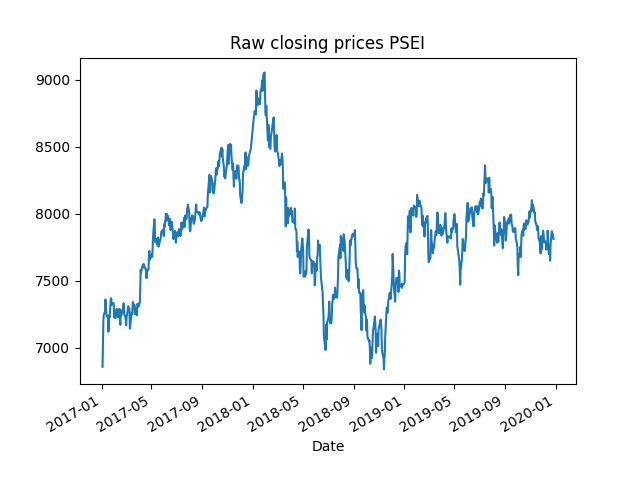
\includegraphics{raw.png}
			\end{figure}
			
		\subsection{Data Preparations}
			Logarithmic returns are  essential in analyzing market volatility as it has properties that arithmetic returns lacks mainly that it is compounding and time-additive properties makes the returns on a financial instrument be non arithmetic based that has complications in return computations \parencite{kitov_log_return}
			
			to attain the logarithmic returns of a financial instrument relevant to the study we have it as such that: $r_t = \ln{\frac{P_t}{P_{t-1}}}$ where $r_t$ is the logarithmic return at that time and $P_t$ is the closing price at that current time and $P_{t-1}$ is the closing price at the time before in the time series \parencite{kitov_log_return}. 
			
			\begin{figure}[htpb]
				\label{fig: log returns_PSEI}
				\caption{Logarithmic Returns of PSEI (January 2017 - December 2019)}
				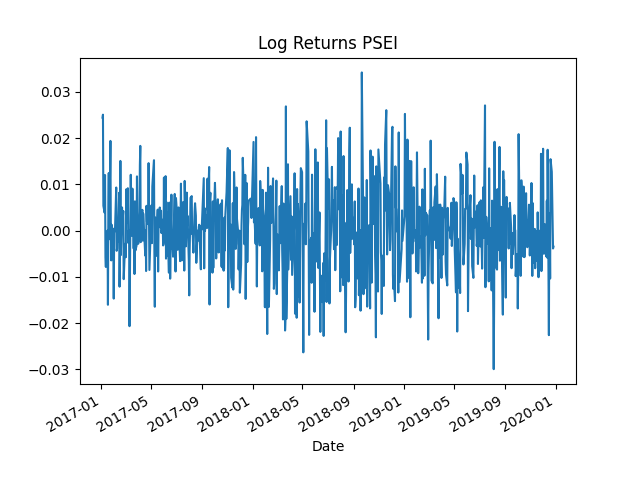
\includegraphics{log_returns.png}
			\end{figure}
			
		\subsection{Rolling Standard Deviation as a Volatility Regime Detection system}
			Volatility in financial time series is estimated using the rolling standard deviation of log returns.
			The rolling standard deviation assesses market volatility dynamically by measuring the
			variability of returns over a shifting time range.
			
			The rolling standard deviation over time $t$ is calculated as the sample standard deviation of log returns inside a window of size $n$.
			
			\begin{equation}
				\sigma_t = \sqrt{\frac{\sum_{i=t-n+1}^{t} {(r_i-\bar{r_i})^2}}{n-1}}
			\end{equation}
			
			where $\bar{r_i}$ is the mean log returns within the given n window of unit of time in the time series data, and $\sigma_t$ is the estimated volatility at that given time \parencite{vipond_standard_deviation}.
		
		\subsection{Short Time Fourier Transform as a Volatility Regime Detection System}
			Traditional Fourier Transforms describe the frequency components in a signal averaged over all time. However in some instances frequency components evolve over time. Short-Time Fourier Transforms enables us to characterize signals with time-varying frequency components \parencite{stern_stft_notes}. Financial markets have closing prices that are non stationary and changes their statistical properties over time STFT can help us identify where does the financial market's certain asset changes its volatility regime or the variance in its closing prices.
			
			The STFT considers only a fixed duration segment of a longer signal and computes its Fourier Transform. This can be done by multiplication of longer time function $x[t]$ and a window function and $\omega[\tau]$ that is brief in duration. Together this creates a rectangular window. If the continuous frequency variable $\omega$ then STFT can be described as:
			\begin{equation}
				X(\tau,\omega) = \int_{\infty}^{-\infty} x(t) \omega(t - \tau) e^{-i \omega t}  dt
			\end{equation}
			
			where $X(\tau, \omega)$ is a complex number that is a function of both time and frequency domains. the $\tau(t)$ is the location of the analysis across the time axis and $\omega$ is the frequency bin the $\omega(t - \tau)$ puts the frequency bin around time $\tau$ \parencite{stern_stft_notes}. the complex exponential form of $	e^{-i \omega t}$ turns projects this time and frequency signal onto a complex sinusoids of:
			\begin{equation}
				e^{-i \omega t} = cos(\omega t) - i sin(\omega t)
			\end{equation}
			this part of the integration turns this into a complex valued function \parencite{Smith1997}.
			
			The extracted feature $X(\tau, \omega)$ is to be squared to be turned onto a STFT Spectogram. A spectogram is the normalized squared magnitude of the STFT coefficients this allows the observation on observations on how the signal changes over time \parencite{stern_stft_notes}.
			
		\subsection{Volatilty Regime Detection}
			Volatility regimes were classified using the 30th and 70th percentile of each method's output as thresholds. Days falling below the 30th percentile were labeled Low, between the 30th and 70th as Medium, and above the 70th as High.
		
		\subsection{Comparing the performance of the STFT against Rolling Standard Deviation}
			A confusion matrix is defined as a table used to visualize the performance of a classifier, with rows and columns representing each class, where each entry indicates the number of cases where a sample was classified as a particular label. It usually contains frequencies. a perfect classifier is  along the diagonal \parencite{sd_confusion_matrix}.
			
			Cohen’s Kappa (k) is used to assess the degree of agreement between two classification methods, while taking into account any chance of agreement.t also allows a more reliable assessment of categorization performance, particularly when
			dealing with unbalanced data or many categories, as in volatility regimes.
			To compute the Cohen's Kappa between STFT and Rolling standard deviation then:
			\begin{equation}
				k = \frac{P_0 - P_e}{1 - P_e}
			\end{equation}
			where $P_0$ is the observed agreement between the two and $P_e$ is the expected agreement by chance
			where $1 \leq K$ or K close to 1 indicates a degree of agreement relative to proximity to 1, 0 indicates all agreements are by chance and anything less than one might be disagreements \parencite{numiqo_cohens_kappa}.
			
			Pearson's R is used to assess the linear relationship between volatility signals created from
			rolling standard deviations and those obtained by STFT. I t measures the strength of relationship between pairs of continuous variables \parencite{kent_pearson_correlation}.
			\begin{equation}
				r = \frac{\sum (x_i - \bar{x})(y_i - \bar{y})}{\sqrt{\sum (x_i - \bar{x})^2 \sum (y_i - \bar{y})^2}}
			\end{equation}
			where $x_i$ is the values from rolling standard deviation, $y_i$ values of the STFT and $\bar{x}$ and $\bar{y}$ is the mean values of the two.
			
	\section{Results}
		\subsection{64  window}
			The 64 day window of both STFT and rolling standard deviation shows significant agreement with one another as shown in \ref{tab:correlation_64day} a correlation score of 0.93 a near perfect correlation implying a strong classification matches between the two systems.
			
			\begin{table}[htbp]
				\centering
				\caption{Pearson correlation for 64 day window}
				\label{tab:correlation_64day}
				\begin{tabular}{@{}lr@{}}
					\hline
					\textbf{Measure} & \textbf{Value} \\
					\hline
					Pearson R & 0.930868203 \\
					\hline
				\end{tabular}
			\end{table}
			
			The confusion matrix shows a large portion of agreement between the two systems with the diagonal being $85.69$ percent of the whole table with the transitions between the regimes the outer ones of the diagonal being the $14.86$ percent of the table showing most of the disagreements being on the transition periods of Low to Medium, Medium to low indicating transition lag for the STFT.
			
			\begin{table}[htbp]
				\centering
				\caption{Confusion matrix comparing STFT volatility regime (rows) to Rolling STDDEV (columns) for 64 day window}
				\label{tab:confusion_64day}
				\begin{tabular}{@{}l r r r@{}}
					\hline
					& \textbf{Low} & \textbf{Medim} & \textbf{High} \\
					\hline
					\textbf{Low}    & 168 & 32  & 0   \\
					\textbf{Medium} & 32  & 218 & 16  \\
					\textbf{High}   & 0   & 16  & 184 \\
					\hline
				\end{tabular}
			\end{table}
			
			The measure of their agreements shows substantial agreement indicating for a long window computations the rolling standard deviation and STFT exhibits the almost the same performance.
			
			\begin{table}[htbp]
				\centering
				\caption{Cohen's kappa statistics and agreement measures for 64 day window}
				\label{tab:kappa_64day}
				\begin{tabular}{@{}l r@{}}
					\hline
					\textbf{Statistic} & \textbf{Value} \\
					\hline
					Agreements & 570 \\
					Disagreements & 96 \\
					N & 666 \\
					Observed Agreement & 0.855855856 \\
					Expected Agreement & 0.339880421 \\
					k & 0.781639344 \\
					Conclusion & Substantial Agreement \\
					\hline
				\end{tabular}
			\end{table}
			
			The figure \ref{fig:chart_64_norm} showed interesting insights as it can be seen that rolling standard deviation being concerned mainly on how far the the window's closing prices are to their mean exhibits many short term micro movements but in the long term tends to be smooth.
			
			\begin{figure}[htbp]
				\label{fig:chart_64_norm}
				\caption{Normalized comparisons of the two volatility regime detection systems under a day window 64}
				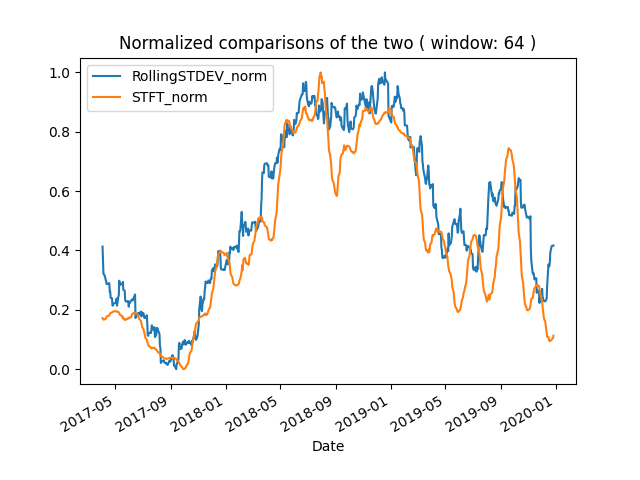
\includegraphics{Normalized_comparisons_two(64).png}
			\end{figure}
			
			The graph for rolling standard deviation \ref{fig:chart_64_sttdev} shows marginal micro movements that is not signinificant enough to shift the market regime classifications under its own system. But is indicative of the nature of its system being mainly concerned with how far does the incoming closing prices are to the mean of the window hence the micro movements since this is non stationary and it is always trying to find the current statistical properties of the said financial instrument where a stationary rolling standard deviation will converge and smooth out from multiple entries this one will not. 
			
			\begin{figure}[htbp]
				\label{fig:chart_64_sttdev}
				\caption{Classifications and readings of Rolling STDEV under a 64 day window}
				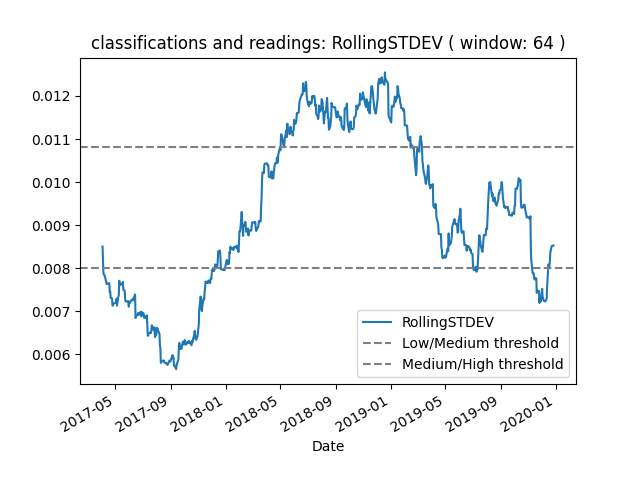
\includegraphics{classifications_and_readings_RollingSTDEV(64).png}
			\end{figure}
			
			The graph for STFT in \ref{fig:chart_64_stft} shows the difference where STFT is mainly concerned with the frequency of the closing prices in its window and is concerned with differentiating what is noise and what is a highly probable intensity of closing price movements deviating from the given window giving it a very smoothed out line due to relatively high number of observations in each window being 64 continuous trading days of closing prices of the PSEI.
			
			\begin{figure}[htbp]
				\label{fig:chart_64_stft}
				\caption{Classifications and readings of STFT under a 64 day window}
				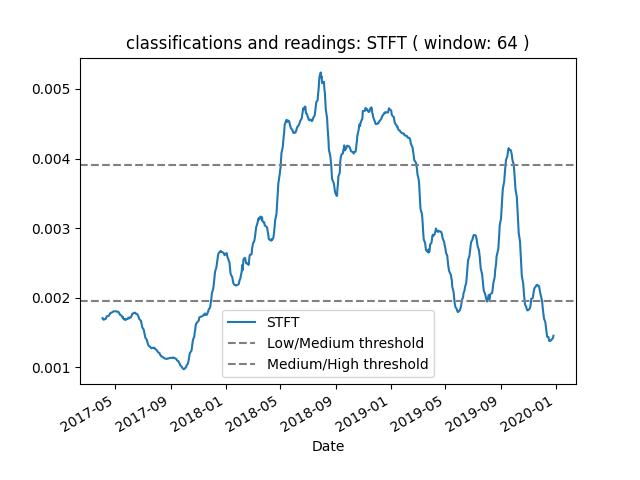
\includegraphics{classifications_and_readings_STFT(64).png}
			\end{figure}
			
			Overall the 64 day window exhibits the long term performance of STFT against Rolling standard deviation and it numerically and visually tracked to the same direction and classifications the relatively large amounts of observations likely helped this convergence. Though there are concerns on the late divergence of the two during the 2020s pandemic as STFT miscalculated a market stabilizing with their lower and lower spectogram yields but is essentially a calm before the storm scenario of pandemic era market stress event.
			
		\subsection{32 day window}
			We can observe a slight breakdown of agreement between the two systems as the correlation coefficient drops to $0.85$. Still a significant commonality in their performance but a more likely disagreements and opposing instances.
		
			\begin{table}[htbp]
				\centering
				\caption{Pearson correlation for 32 day window}
				\label{tab:correlation_32day}
				\begin{tabular}{@{}lr@{}}
					\hline
					\textbf{Measure} & \textbf{Value} \\
					\hline
					Pearson R & 0.85283811 \\
					\hline
				\end{tabular}
			\end{table}
			
			The confusion matrix now that their windows have narrowed also worsened as the diagonals their agreements became worst to $76.79$
			percent indicating that STFT follows the rolling standard deviation calculations less the less information there are as their disagreements becomes $23.20$ percent of the matrix.
			
			\begin{table}[htbp]
				\centering
				\caption{Confusion matrix comparing STFT volatility regime (rows) to Rolling STDDEV (columns) for 32 day window}
				\label{tab:confusion_32day}
				\begin{tabular}{@{}l r r r@{}}
					\hline
					& \textbf{Low} & \textbf{Medim} & \textbf{High} \\
					\hline
					\textbf{Low}    & 156 & 54  & 0   \\
					\textbf{Medium} & 54  & 197 & 27  \\
					\textbf{High}   & 0   & 27  & 183 \\
					\hline
				\end{tabular}
			\end{table}
			
			The two systems under a medium-term 32 day window still exhibits a substantial agreement though the strength of this agreement is tested more as it is weaker now.
			
			\begin{table}[htbp]
				\centering
				\caption{Cohen's kappa statistics and agreement measures for 32 day window}
				\label{tab:kappa_32day}
				\begin{tabular}{@{}l r@{}}
					\hline
					\textbf{Statistic} & \textbf{Value} \\
					\hline
					Agreements & 536 \\
					Disagreements & 162 \\
					N & 698 \\
					Observed Agreement & 0.767908309 \\
					Expected Agreement & 0.309430957 \\
					k & 0.648527 \\
					Conclusion & Substantial Agreement \\
					\hline
				\end{tabular}
			\end{table}
			
			The side-by-side normalized comparison of STFT and rolling standard deviation at \ref{fig:chart_32_norm} still shows general long term agreeableness between the two systems with rolling standard deviation and STFT starting to have a lot of jigsaw movements due to the narrowing of observations the two systems can calculate from based on their rolling windows. With STFT's sharper movements being more noticeable as it is referencing from smaller frequency observations and will be less conservative against the older spectogram observations it made in the older parts of its rolling window.
			
			\begin{figure}[htbp]
				\label{fig:chart_32_norm}
				\caption{Normalized comparisons of the two volatility regime detection systems under a day window 32}
				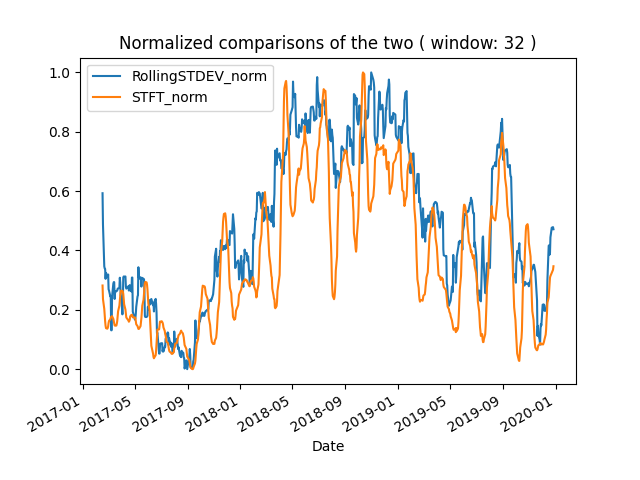
\includegraphics{Normalized_comparisons_two(32).png}
			\end{figure}
			
			The rolling standard deviation system under a 32 day window is starting to show more drastic movements that is borderline on both its volatility regime threshold line exhibiting several false impressions of transitions to a certain volatility regime but in the long term is actually going in the opposing way in terms of closing prices volatility.
			
			\begin{figure}[htbp]
				\label{fig:chart_32_sttdev}
				\caption{Classifications and readings of RollingSTDEV under a 64 day window}
				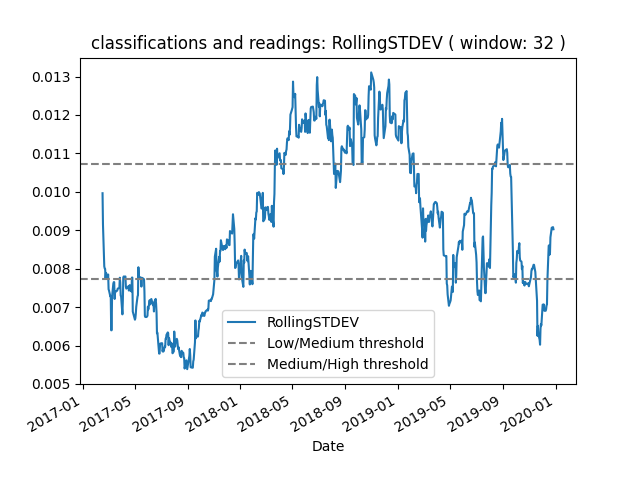
\includegraphics{classifications_and_readings_RollingSTDEV(32).png}
			\end{figure}
			
			The STFT system under a 32 day window exhibits more sharper spectogram movements than before to be expected as it has less more past frequencies to compare incoming spectogram entries allowing for more sensitivity to newer entries. This increase in sensitivity allowed it to catch medium term closing prices movements and allows it to be as responsive as rolling standard deviation system in the medium term.
			
			\begin{figure}[htbp]
				\label{fig:chart_32_stft}
				\caption{Classifications and readings of STFT under a 32 day window}
				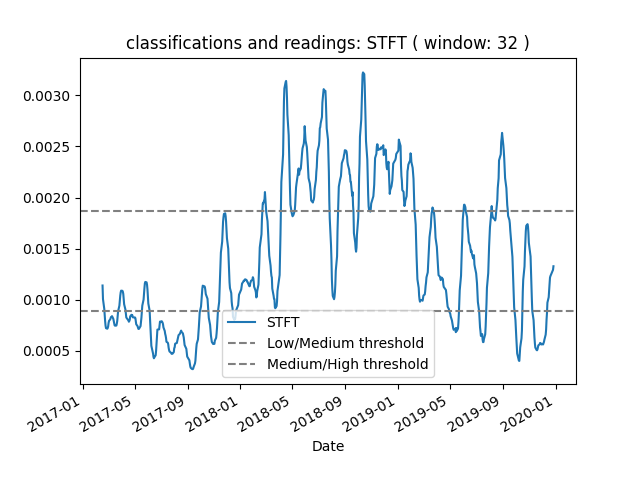
\includegraphics{classifications_and_readings_STFT(32).png}
			\end{figure}
			
			The two systems in the medium term of a 32 day window has more disagreements now than before which is expected with a much lower rolling window data to compute against. The two numerically and visually do generally agree with each other on volatility regime classifications with disagreements mainly in classification timings.

		\subsection{16 day window}
		The further narrowing of their window shows further breakdowns in their agreements as the narrower source of information influences the performance of STFT against rolling standard deviation with a correlation coefficient of $0.807239$.
		
		\begin{table}[htbp]
			\centering
			\caption{Pearson correlation for 16 day window}
			\label{tab:correlation_16day}
			\begin{tabular}{@{}lr@{}}
				\hline
				\textbf{Measure} & \textbf{Value} \\
				\hline
				Pearson R & 0.807239 \\
				\hline
			\end{tabular}
		\end{table}
		
		Their confusion matrix became worst as the diagonal agreement now only composed of $71.98$ a noticeable decline in similarity of performance with their disagreements being $28.01$ percent with a noted Low STFT volatility regime and High rolling standard deviation wrong classifications present.
		
		\begin{table}[htbp]
			\centering
			\caption{Confusion matrix comparing STFT volatility regime (rows) to Rolling STDDEV (columns) for 16 day window}
			\label{tab:confusion_16day}
			\begin{tabular}{@{}l r r r@{}}
				\hline
				& \textbf{Low} & \textbf{Medium} & \textbf{High} \\
				\hline
				\textbf{Low}    & 165 & 47  & 2   \\
				\textbf{Medium} & 49  & 187 & 50  \\
				\textbf{High}   & 0   & 52  & 162 \\
				\hline
			\end{tabular}
		\end{table}
		
		The breakdown of agreement between the two systems can be seen here at Cohen's Kappa as their agreement got rated as moderate.
		
		\begin{table}[htbp]
			\centering
			\caption{Cohen's kappa statistics and agreement measures for 16 day window}
			\label{tab:kappa_16day}
			\begin{tabular}{@{}l r@{}}
				\hline
				\textbf{Statistic} & \textbf{Value} \\
				\hline
				Agreements & 514 \\
				Disagreements & 200 \\
				N & 714 \\
				Observed Agreement & 0.719887955 \\
				Expected Agreement & 0.295718287 \\
				k & 0.575514 \\
				Conclusion & Moderate Agreement \\
				\hline
			\end{tabular}
		\end{table}
		
		The comparative graph observed in \ref{fig:chart_16_norm} shows extreme whipsaws on both systems. With STFT having extreme movements due to having the narrowest amount of spectograms to measure incoming ones. Leading to a lot of incomprehensible changes that can be high volatility regime one time and then low volatility regime in the succeeding time. Both systems do still visually follow one another but it is less visible than ever.
		
		\begin{figure}[htbp]
			\label{fig:chart_16_norm}
			\caption{Normalized comparisons of the two volatility regime detection systems under a day window 16}
			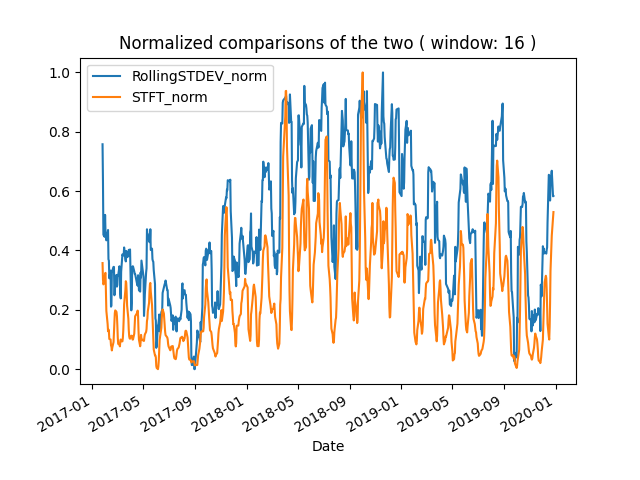
\includegraphics{Normalized_comparisons_two(16).png}
		\end{figure}
		
		The rolling standard deviation system under a 16 day rolling window as seen in \ref{fig:chart_16_sttdev}. what is notable is the convergence of movements of it are now outside the threshold lines and the narrowing of the medium transition zone in between the high market volatility regime threshold and low market volatility regime detection line as this narrowing signifies that a quantile of $0.3$ and $0.7$ might be insufficient to catch geniune volatility regime changes and a more extreme values is to be considered at a narrow window.
		
		\begin{figure}[htbp]
			\label{fig:chart_16_sttdev}
			\caption{Classifications and readings of RollingSTDEV under a 16 day window}
			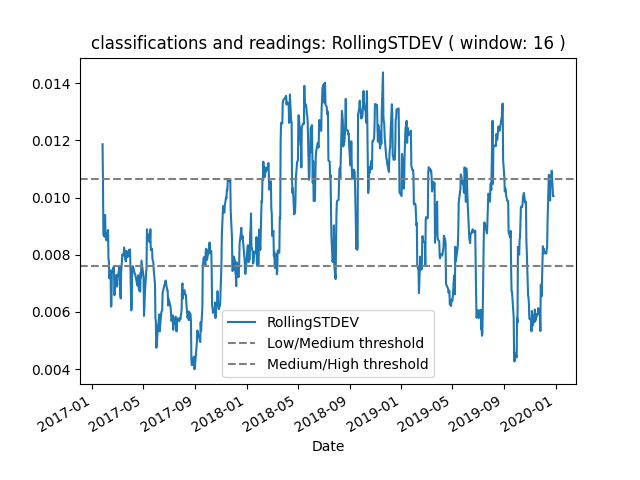
\includegraphics{classifications_and_readings_RollingSTDEV(16).png}
		\end{figure}
		
		The STFT system under a 16 day rolling window as seen in \ref{fig:chart_16_sttdev} exhibits the limitations of using a single quantile to determine volatility regime detection as the transition zone is ill suited for the amount of swings the STFT computations provided to determine credible volatility regime shifts as the most swings just breaches the region instead of what was observed in larger windows where the transition region signifies the PSEI might be in transition from stable low closing prices movements to a more high volatile regime of strong upward price direction or much more extreme closing price downstream.
		
		\begin{figure}[htbp]
			\label{fig:chart_16_stft}
			\caption{Classifications and readings of STFT under a 32 day window}
			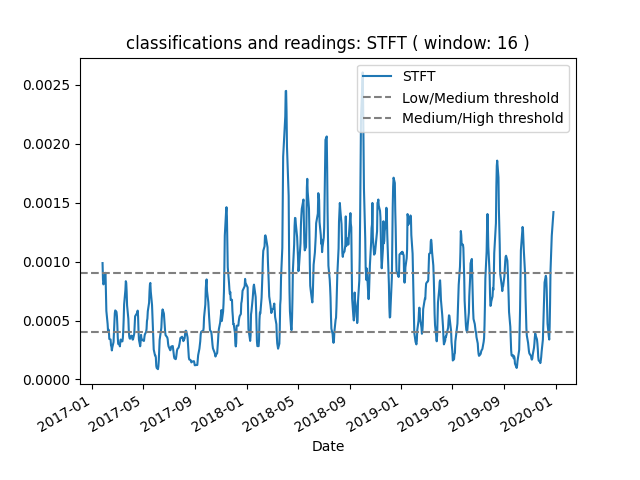
\includegraphics{classifications_and_readings_STFT(16).png}
		\end{figure}
		
		Overall while there is still notable agreeableness between the two systems the narrower rolling window is starting to decouple the similarities in the performance of the two.
		
		
	\section{Discussion}
		The study’s results show a strong relationship between the STFT-based volatility regime classification and the classical rolling standard deviation approach, especially in the context of the 64-day window. Since the Pearson correlation coefficient (r = 0.9309) shows a very high positive correlation, these results suggest that both methods capture similar volatility relationship over longer time horizons. 
		
		This is also further supported by the confusion matrix, as we see a considerable number of observations that lie along the diagonal (Low–Low, Medium–Medium, High–High), meaning consistent classification between the two methods is not random but systematic. Moreover, the Cohen’s kappa value ( k = 0.7816) indicates substantial agreement, reinforcing the reliability of the observed consistency.
		
		With respect to the 32-day window, we still get a strong Pearson correlation (r = 0.8528), but it is much weaker than for the 64-day window. It implies that the two methods become slightly less congruent as the observation window reduces. Shorter windows tend to have increased sensitivity to sudden spikes in volatility, which can introduce variance and decrease consistency between the classification types. 
		
		Visual comparisons between the two systems shows that while numerically they are almost the same in their classification performances. They have variations on when and where they switch classifications of market volatility as STFT is more later in their shifts than the rolling standard deviation due to the system being more concerned on the general trend of the frequencies than they are at the distance to the mean of the new entries of the rolling window.
		
		This much more smoothed and laggard classification system allows STFT to have lesser early false indications on regime switching than rolling standard deviation. Though it is more comprehensible on medium term 32 days rolling window and 64 days rolling window where the much larger observations within the window itself allows more removal of short term noises and jigsaw movements prevalent with 16 and lesser days rolling windows.
		
		Yet there are some discrepancies, especially within neighbouring categories like Low–Medium and Medium–High ones. These misclassifications are likely due to the greater sensitivity of the STFT method to short-term fluctuations than that of the rolling standard deviation, which may cause slightly differing regime boundary locations. That suggests that although both are consistent in general, STFT could register more localized volatility changes that are less pronounced in rolling measures.
		
		The study is limited in scope as what counts as short term and long term depends largely on the makers of their financial modeling systems meant to fit their broader market strategies. The 64, 32, 16 days rolling window might not be relevant or highly relevant depending on the time frames of the analysis needed.
		It is also only tested with the daily closing prices of the PSEI and other emerging markets might have different statistical properties that is not relevant to PSEI that the two systems might diverge or converge against it is highly recommended to not take the findings at face value when applying it to non PSEI markets or more developed financial markets of the world.
		
		Overall, the findings indicate that the STFT-based approach is a valid alternative to rolling standard deviation for volatility regime detection, especially over longer time frames, as it maintains high correlation and substantial agreement while also capturing short-term dynamics in volatility behavior.
		
	\section{Conclusion}
		This study has shown that the Short-Time Fourier Transform (STFT) is a reliable and efficient technique for identifying volatility regimes in the Philippine Stock Exchange Index (PSEI) between 2017 and 2019. STFT yielded results that were largely consistent across all window widths when compared to the rolling standard deviation technique, with the 64-day window showing the highest agreement. Specifically, the 64-day window produced the strongest Cohen's kappa and Pearson correlation, showing that both approaches closely followed one another and categorized volatility regimes in a very comparable manner. While the 16-day window only shown moderate agreement, the 32-day window still demonstrated significant agreement, indicating that the resemblance between the two approaches diminishes as the observation window gets shorter.
		
		
		Because STFT captures the overall shift of volatility regimes while staying sensitive to time-varying changes in market behavior, the results also imply that it is particularly helpful for longer-term volatility studies. However, compared to rolling standard deviation, STFT became more susceptible to sudden changes at shorter windows, which resulted in more discrepancies in classification time. This indicates that when the analysis window is too small, STFT's performance becomes less steady even though it can identify localized changes in volatility.
		
		Overall, the study finds that, especially when longer rolling windows are employed, STFT can be a potent substitute for rolling standard deviation in identifying volatility regimes in an emerging market like the Philippine stock market. The findings validate the application of STFT in financial volatility research and indicate that further testing of larger datasets, different threshold settings, and other market periods, particularly during significant financial shocks may enhance regime recognition even more.
		
	\printbibliography
	
	\appendix
	
	\section{Appendix A: readings(16).csv (raw dump)}
	\begin{verbatim}
		confusion matrix,"[[165  47   2]
		[ 49 187  50]
		[  0  52 162]]"
		"volatility threshold stddev (low, high)",
		"[np.float64(0.00759471350903402), np.float64(0.010661367061913247)]"
		"volatility threshold stft (low, high)",
		"[np.float64(0.0004036449411981957), np.float64(0.0009050641462424594)]"
		cohen's kappa,0.5755154455304273
		correlation coefficient,0.8072397868737419
		p value,3.404328307344355e-165
	\end{verbatim}
	
	\section{Appendix B: readings(32).csv (raw dump)}
	\begin{verbatim}
		confusion matrix,"[[156  54   0]
		[ 54 197  27]
		[  0  27 183]]"
		"volatility threshold stddev (low, high)",
		"[np.float64(0.007735338831005285), np.float64(0.010718554270557139)]"
		"volatility threshold stft (low, high)",
		"[np.float64(0.0008851187089477077), np.float64(0.0018655799357252163)]"
		cohen's kappa,0.648526669153301
		correlation coefficient,0.8528381100263377
		p value,1.4112544500705062e-198
	\end{verbatim}
	
	\section{Appendix C: readings(64).csv (raw dump)}
	\begin{verbatim}
		confusion matrix,"[[168  32   0]
		[ 32 218  16]
		[  0  16 184]]"
		"volatility threshold stddev (low, high)",
		"[np.float64(0.008001526264052296), np.float64(0.01080491316888701)]"
		"volatility threshold stft (low, high)",
		"[np.float64(0.001956248855256931), np.float64(0.003907888473774559)]"
		cohen's kappa,0.7816393442622951
		correlation coefficient,0.9308682033623458
		p value,1.4609033148661047e-292
	\end{verbatim}
	
\end{document}